\chapter{Literature Review}
\label{chap:lit.review}

\section{Introduction}

\subsection{Recurrent Neural Networks}

Recurrent Neural Networks (RNNs) are in forefront of recent development and advances in \textit{deep learning} by making able neural networks to deal with sequences data, which is a major shortcoming in ANN. If the data is based on sequence of events in a video or text, the traditional neural network can't do reasoning for a single event based on its previous one. To tackle this issue RNNs have loops which enables them to persist the information.

\begin{figure}[p]
	\centering
	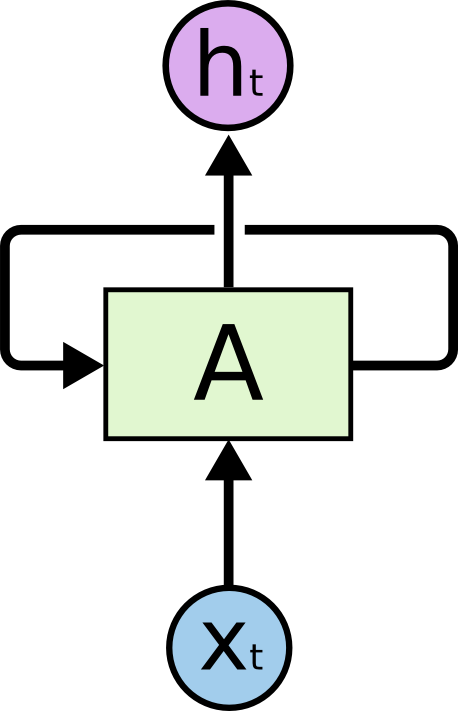
\includegraphics[scale=0.4]{./figs/rnn-rolled}
	\caption[A Rolled Recurrent Neural Networks]{Recurrent Neural Networks (RNNs) uses loops.}
	\label{fig:rnn-rolled}
\end{figure}

As it shown in \textbf{Figure \ref{fig:rnn-rolled}}, a selected neural network, $A$ takes the input $x_t$ and outputs the value of $h_t$. this might not show how data goes from one step to the next one in a same network until you unroll the loop and see chain architecture of recurrent neural networks that makes them the best choice for sequential data, \textbf{Figure \ref{fig:rnn-unrolled}}.

\begin{figure}[p]
	\centering
	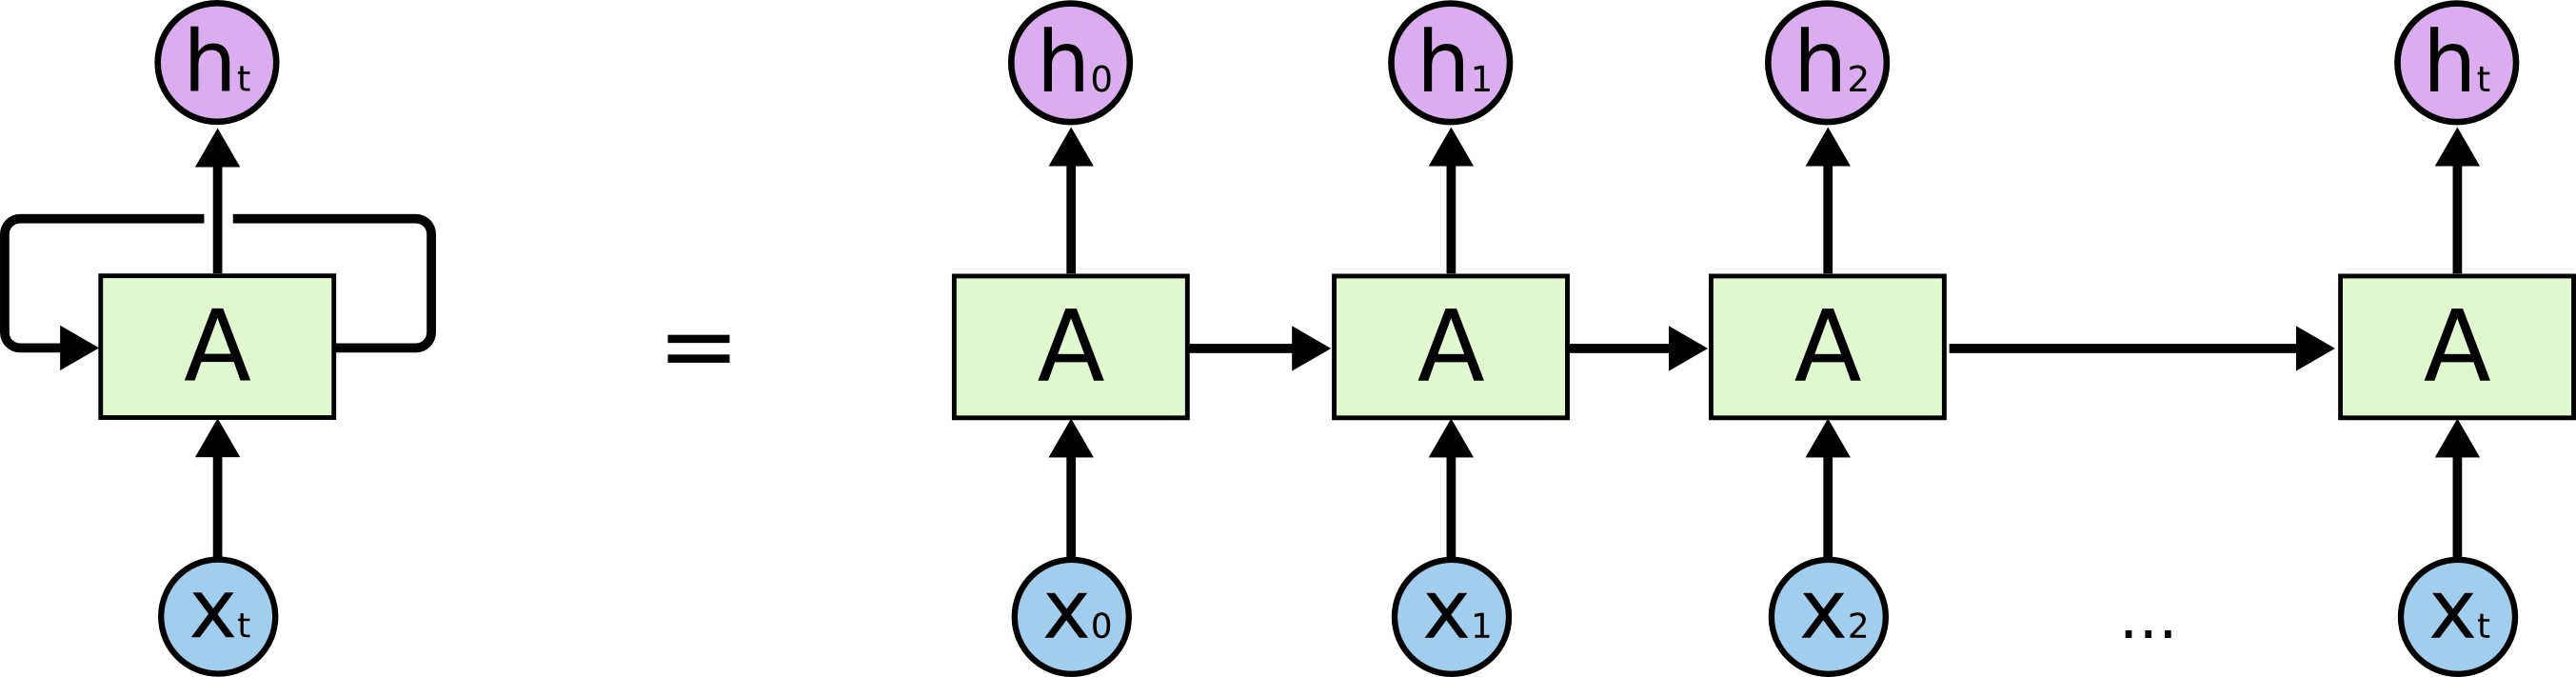
\includegraphics[scale=0.4]{./figs/rnn-unrolled}
	\caption[An Unrolled Recurrent Neural Networks]{An Unrolled Recurrent Neural Networks (RNNs).}
	\label{fig:rnn-unrolled}
\end{figure}

While RNNs is being used in variety of applications from language modeling to image captioning, the essential to all these achievement is the RNN-LSTMs \cite{Hochreiter1997}. An enhanced version of RNNs that outperforms better than the standard RNN.

\subsection{Bayes by Backprop}

Bayes by Backprop \cite{Blundell2015a} is a variational inference scheme for learning the posterior distribution on the weights of a neural network.
The posterior distribution on parameters of the network $\theta \in \mathbb{R}^d$, $q(\theta)$ is typically taken to be a Gaussian with mean parameter $\mu\in \mathbb{R}^d$ and standard deviation parameter $\sigma\in \mathbb{R}^d$, denoted $\mathcal{N}(\theta|\mu,\sigma)$ and it's a diagonal covariance matrix. Where $d$ is the dimensionality of the parameters of the network (usually refers to scale of millions).
Let $\log p(y|\theta, x)$ be the log-likelihood of the neural network, then the network is trained by minimising the variational free energy, where $p(\theta)$ is a prior on the parameters:

\begin{align}
	\label{eq:elbo}
	\mathcal{L}(\theta) &=
	\mathbb{E}_{q(\theta)}\left[\log \frac{q(\theta)}{p(y|\theta, x)p(\theta)}\right],
\end{align}

The \textbf{algorithm \ref{alg:bbb}} shows the Bayes by Backprop Monte Carlo procedure for minimising the above equation with respect to the mean and standard deviation parameters of the posterior $q(\theta)$.

Minimising the variational free energy equation is equivalent to maximising the log-likelihood $\log p(y|\theta, x)$ subject to a KL complexity term in the parameters of the network that acts as a regulariser:

\begin{align}
	\label{eq:klelbo}
	\mathcal{L}(\theta) &=
	- \mathbb{E}_{q(\theta)}\left[\log p(y|\theta, x) \right]
	+ \kl{q(\theta)}{p(\theta)}.
\end{align}

Gaussian process in a case with zero mean prior, the KL term acts as a form of weight decay on the mean parameters, where the rate of weight decay is automatically tuned by the standard deviation parameters of the prior and posterior.

\begin{algorithm}[ht]
	\caption{Bayes by Backprop}
	\label{alg:bbb}
	\begin{algorithmic}
		\STATE{Sample $\epsilon \sim \mathcal{N}(0, I)$, $\epsilon \in \mathbb{R}^d$.}
		\STATE{Set network parameters to $\theta = \mu + \sigma\epsilon$.}
		\STATE{Do forward propagation and backpropagation as normal.}
		\STATE{Let $g$ be the gradient with respect	\label{eq:elbo}
			\mathcal{L}(\theta) &=
			\mathbb{E}_{q(\theta)}\left[\log \frac{q(\theta)}{p(y|\theta, x)p(\theta)}\right], to $\theta$ from backpropagation.} 
		\STATE{Let $g^{KL}_\theta, g^{KL}_\mu, g^{KL}_\sigma$ be the gradients of $\log \mathcal{N}(\theta|\mu, \sigma) - \log p(\theta)$ with respect to $\theta$, $\mu$ and 
			$\sigma$ respectively.} 
		\STATE{Update $\mu$ according to the gradient $g + g^{KL}_\theta + g^{KL}_\mu$.} 
		\STATE{Update $\sigma$ according to the gradient $(g + g^{KL}_\theta) \epsilon + g^{KL}_\sigma$.}
	\end{algorithmic}
\end{algorithm}

The uncertainty afforded by Bayes by Backprop trained networks has been used successfully for training feed-forward NN models for supervised learning and also to help exploration to reinforcement learning agents \cite{Blundell2015a}, \cite{Lipton2016}, \cite{Houthooft2016}, but until now, BBB has not been applied to recurrent neural networks.




\subsection{Model Confidence}

\subsection{Model Uncertainty and Safety}

\section{State-of-the-Arts}

Sharpening the posterior as proposed in Chapter \ref{chap:method} has mutualities with other techniques. Such as line search, where $\eta$ is a trained parameter that does line search along the gradient direction to give probabilistic interpretations to line search. In this work the novel technique is to use a variational posterior with the reparametrization gradient.

Another similar technique is dynamic evaluation \cite{Mikolov2010}, which trains an RNN during evaluation of the model with a fixed learning rate. The update applied in this case is cumulative, and only uses previously seen data. Thus, they can take a purely deterministic approach and ignore any KL between a posterior with privileged information and a prior.

Lastly, learning to optimise (or learning to learn) \cite{Li2016a} is related in that a learning rate is learned so that it produces better updates than those provided by e.g. AdaGrad \cite{Duchi2011} or Adam \cite{Kingma2013a}. Whilst they train a parametric model, we treat these as free parameters (so that they can adapt more quickly to the non-stationary distribution w.r.t. parameters). Notably, we use gradient information to inform a variational posterior so as to reduce variance of Bayesian Neural Networks. Thus, although similar in flavour, the underlying motivations are quite different.

Applying Bayesian methods to neural networks has a long history, with most common approximations having been tried.
\citet{buntine1991bayesian} propose various maximum a posteriori schemes for neural networks, including an approximate posterior
centered at the mode.
\citet{buntine1991bayesian} also suggest using second order derivatives in the prior to encourage smoothness of the resulting network.
\cite{Hinton1993} proposed using variational methods for compressing the weights of neural networks as a regulariser.
\cite{Hochreiter1995} suggest an MDL loss for single layer networks that penalises non-robust weights by means of an approximate penalty based upon perturbations of the weights on the outputs.
\cite{Mackay1995} investigated using the Laplace approximation for capturing the posterior of neural networks.
\citet{neal2012bayesian} investigated the use of hybrid Monte Carlo for training neural networks, although it has so far been difficult to apply these to the large sizes of networks considered here.

More recently \citet{graves2011practical} derived a variational inference scheme for neural networks and
\cite{Blundell2015a} extended this with an update for the variance that is unbiased and simpler to compute.
\cite{Graves2016} derives a similar algorithm in the case of a mixture posterior.
Several authors have claimed that dropout \cite{Srivastava2014} and Gaussian dropout \cite{Wang2013} can be viewed as approximate variational inference schemes \cite{Gal2015}, \cite{Kingma2015}.
\cite{Gan2016} goes a step further and uses Monte Carlo dropout for LSTMs (we compare to this results in our experiments).
Variational methods typically underestimate the uncertainty in the posterior (as they are mode seeking, akin to the Laplace approximation), whereas expectation propagation methods are mode averaging and so tend to overestimate uncertainty.
Nonetheless, several papers explore applying expectation propagation to neural networks:
\cite{Soudry2014} derive a closed form approximate online expectation propagation algorithm, whereas \citet{hernandez2015probabilistic} proposed using multiple passes of assumed density filtering (in combination with early stopping) attaining good performance on a number of small data sets.
\citet{hasenclever2015distributed} derive a distributed expectation propagation scheme with SGLD \cite{Welling2011} as an inner loop.
Others have also considered applying SGLD to neural networks \citep{li2015preconditioned} and \cite{Gan2016} more recently used SGLD for LSTMs (we compare to these results in our experiments).

\section{Limitations}
\begin{enumerate}
\item Mentor~Graphics 2
\begin{enumerate}
\item item 3
\end{enumerate}
\item item 4
\end{enumerate}

\section{Research Gaps}
The processing at layer-5%
